\documentclass{report}
\usepackage{float}
\usepackage[utf8]{inputenc}
\usepackage[T1]{fontenc}
\usepackage{geometry}
\usepackage{hyperref}
\usepackage{amsmath}
\usepackage{graphicx}
\usepackage{listings}
\usepackage{xcolor} % Pour la coloration syntaxique
\geometry{margin=1in}
\graphicspath{{./img/}}
\makeindex

%================== Required Packages ===================%
\usepackage{tcolorbox}       % For colored boxes
\usepackage{afterpage}       % To execute commands after the current page
\usepackage{array,longtable,multirow} % For advanced table formatting
\usepackage{pifont}          % For special symbols (e.g., checkmarks, crosses)
\usepackage{pdflscape}       % For landscape pages in PDF
\usepackage{rotating}        % For rotating text and figures
\usepackage{wrapfig}         % For wrapping text around figures
\usepackage[french]{babel}   % For French language support

\usepackage{fontspec} % For font management
\usepackage{arabxetex} % Arabic support for XeLaTeX

\newfontface\montserrat{Montserrat}

\begin{document}

\thispagestyle{empty} % Replace with 'empty' if 'cover' is not defined
\newgeometry{bottom=25mm,left=20mm,top=15mm,right=20mm}

\hspace{-40pt}
\begin{minipage}[c]{0.33\columnwidth} % Center-aligned vertically
    \vspace{6mm}
    \centering
    \begingroup
    \setmainfont{Arimo}
        Ministère de l'Enseignement Supérieur et de la Recherche Scientifique\\
        Institut International de Technologie à Sfax
    \endgroup
\end{minipage}
\hfill % Adds horizontal space between minipages
\begin{minipage}[c]{0.33\columnwidth} % Center-aligned vertically
    
\includegraphics[width=1\columnwidth]{LogoIIT}
\end{minipage}
\hfill % Adds horizontal space between minipages
\begin{minipage}[c]{0.33\columnwidth} % Center-aligned vertically
    \vspace{0mm}
    \centering
    \begin{arab}% Arabic script range
        \textbf{وزارة التعليم العالي والبحث العلمي \\
        المدرسة العليا الدولية الخاصة للتكنولوجيا \\
        بصفاقس
        }
    \end{arab}
    
\end{minipage}
\hspace{-20pt}

\vskip5mm
\hrule

\vskip2.5cm

\begin{center}

\begin{center}
\fontsize{30pt}{1pt}\textbf{
\textsc{Rapport de Projet}
}
\end{center}

\vskip1cm


{\fontsize{12pt}{1pt}


\textcolor[HTML]{114388}{\textrm{Élaboré par : }}
\vskip0.1cm
    \textbf{Chedy Chaaben} \\
    \textbf{Taieb Jemal}
\vskip2cm
}
\begin{tcolorbox}[colframe=black, colback=white, 
    toprule=2pt, bottomrule=2pt, 
    leftrule=0pt, rightrule=0pt, 
    arc=0mm]
    \centering
     {\fontsize{30}{38}\montserrat\textbf{Développement d'une Application de Commande en Ligne pour Restaurant}}
\end{tcolorbox}

\vskip2.5cm

{\fontsize{15pt}{1pt}
\textcolor[HTML]{114388}{\textrm{Enseignant : }}
    \textbf{ M. Fahmi KALLEL}
\vskip2.5cm
}


{\fontsize{18pt}{1pt}
Année universitaire : 2023/2024
}
\end{center}
\newpage

\tableofcontents
\newpage

\chapter*{Introduction générale}
\addcontentsline{toc}{chapter}{Introduction générale} 

\markboth{Introduction générale}{}

Dans un monde de plus en plus connecté et numérique, la gestion efficace des systèmes d'information est essentielle pour garantir la bonne marche des entreprises, y compris celles du secteur de la restauration. L'automatisation des processus, la sécurisation des données et l'amélioration de l'expérience utilisateur deviennent des éléments clés pour répondre aux défis contemporains. Dans ce contexte, la gestion d'un restaurant ne se limite plus à des tâches manuelles, mais s'appuie sur des solutions logicielles intelligentes pour optimiser les opérations quotidiennes, comme la gestion des commandes et du stock des produits.

Ce projet de développement d'une application web pour un restaurant se focalise sur l'utilisation d'une API, offrant ainsi une meilleure flexibilité et sécurité, plutôt que sur un site web traditionnel. 

L'objectif est de permettre une gestion fluide des commandesau sein du système tout en garantissant un accès sécurisé aux différentes fonctionnalités de l'application. 

Afin d’illustrer et de structurer efficacement cette application, des diagrammes de classe et des cas d’utilisation ont été élaborés pour fournir une vue d'ensemble des entités et de leurs interactions dans l’application. En outre, une série d'endpoints API ont été développés pour permettre la communication entre le serveur et le client, facilitant ainsi les opérations de gestion des commandes.

\clearpage

\chapter{Authentification avec JWT (JSON Web Token)}


L'authentification par \textbf{JWT (JSON Web Token)} est une méthode largement utilisée pour sécuriser les API web. Un \textbf{JWT} est un jeton compact et autonome qui permet de transmettre de manière sécurisée des informations entre un client et un serveur sous forme d'un objet JSON. Ce jeton est signé numériquement, généralement avec un algorithme comme HMAC ou RSA, afin de garantir l'intégrité des données et de vérifier l'authenticité de l'émetteur.

L'authentification par JWT est particulièrement adaptée aux systèmes \textbf{stateless}, car elle permet de ne pas avoir besoin de stocker de session côté serveur. En effet, contrairement à une session traditionnelle où des informations sont conservées sur le serveur, le JWT contient toutes les informations nécessaires à l'identification de l'utilisateur et à l'autorisation d'accès aux ressources protégées.

Les principaux avantages de l'utilisation de JWT sont les suivants :
\begin{itemize}
    \item \textbf{Stateless} : Il n'est pas nécessaire de maintenir l'état de la session sur le serveur, ce qui simplifie la gestion de la scalabilité de l'application.
    \item \textbf{Sécurisé} : Le JWT est signé numériquement, ce qui garantit que son contenu n’a pas été modifié et qu’il provient d’une source fiable.
    \item \textbf{Flexible} : Le JWT peut contenir diverses informations utiles, telles que les rôles d’utilisateur, la date d’expiration et d'autres attributs.
\end{itemize}


\section{Structure d’un JWT}

Un JWT se compose de trois parties distinctes, séparées par des points (\texttt{.}) :
\begin{itemize}
    \item \textbf{Header} : Spécifie le type de token (JWT) et l’algorithme de signature utilisé (par exemple, HMAC SHA256 ou RSA).
    \item \textbf{Payload} : Contient les informations ou \textbf{claims}, comme l’ID utilisateur, le rôle de l’utilisateur, et la date d’expiration du token.
    \item \textbf{Signature} : Générée en utilisant le Header, le Payload et une clé secrète partagée entre le client et le serveur, afin de garantir l’intégrité et l'authenticité du jeton.
\end{itemize}

Voici un exemple de structure d'un JWT :
\[
\texttt{<Header>.<Payload>.<Signature>}
\]

\section{Pourquoi utiliser JWT ?}

L'utilisation de JWT présente plusieurs avantages qui en font un choix idéal pour l'authentification et l'autorisation dans les applications modernes :
\begin{itemize}
    \item \textbf{Authentification sans état} : Le serveur n’a pas besoin de stocker de sessions, ce qui simplifie la gestion des ressources et augmente la scalabilité de l’application.
    \item \textbf{Sécurité} : Le jeton est signé numériquement, ce qui garantit son intégrité. Il peut également être chiffré pour protéger les informations sensibles qu'il contient.
    \item \textbf{Flexibilité} : Le JWT permet d'intégrer divers types de données, telles que les rôles ou les permissions, directement dans le jeton, facilitant ainsi la gestion des accès à différentes ressources.
\end{itemize}

\section{Fonctionnement dans l’application}

Voici les étapes du fonctionnement de l’authentification avec JWT dans notre application :

\begin{enumerate}
    \item \textbf{Lors de la connexion de l’utilisateur} : Lorsque l’utilisateur saisit son nom d'utilisateur et son mot de passe dans l'interface de connexion, ces informations sont envoyées au backend via une requête HTTP. Si les informations sont valides, le backend génère un JWT contenant des informations telles que l'ID de l'utilisateur, son rôle et une date d’expiration du jeton. Ce jeton est renvoyé au client.
    
    \item \textbf{Stockage du JWT côté client} : Une fois le JWT généré et renvoyé, le frontend (le client) stocke ce jeton. Dans notre application, le jeton est généralement stocké dans le \texttt{localStorage} du navigateur, bien qu'il soit également possible de l'utiliser dans des cookies pour certaines configurations. Ce stockage permet au client de conserver le jeton entre les sessions et d'envoyer ce jeton pour chaque requête ultérieure.
    
    \item \textbf{Envoi du JWT dans les requêtes suivantes} : Pour chaque requête suivante nécessitant une authentification (par exemple, pour consulter le menu ou passer une commande), le client inclut le JWT dans l’en-tête \texttt{Authorization} de la requête HTTP. Le format de cet en-tête est :
    \[
    \texttt{Authorization: Bearer <token>}
    \]
    
    \item \textbf{Validation du token par le serveur} : À chaque requête, le serveur vérifie la validité du jeton envoyé par le client. Cela se fait à l'aide d'un middleware sur le backend. Ce middleware décode le JWT, vérifie sa signature à l'aide de la clé secrète, et s'assure que le jeton n’a pas expiré. Si le jeton est valide, l'accès à la ressource demandée est accordé. En revanche, si le jeton est invalide ou expiré, le serveur renvoie une erreur d'authentification (généralement avec le code HTTP 401).
\end{enumerate}

\textbf{Résumé du flux d'authentification} :
\begin{enumerate}
    \item L'utilisateur se connecte avec ses identifiants.
    \item Si l'authentification réussit, un JWT est généré et envoyé au client.
    \item Le client stocke ce JWT et l'envoie avec chaque requête suivante.
    \item Le backend valide le token et permet l'accès aux ressources protégées.
\end{enumerate}

Ce flux d’authentification garantit une gestion sécurisée et scalable des utilisateurs dans l'application, sans la nécessité de maintenir des sessions sur le serveur.


\clearpage

\chapter{Repository Pattern}


Le \textbf{Repository Pattern} est un design pattern qui permet de créer une couche d’abstraction entre la logique métier d'une application et la persistance des données, généralement une base de données. Ce modèle se situe entre les couches de logique métier (services) et la couche d’accès aux données (base de données ou autre source de données), et permet de centraliser l’accès aux données dans une ou plusieurs classes appelées "repositories".

L’idée principale du \textbf{Repository Pattern} est de masquer les détails de l’implémentation de l’accès aux données (requêtes SQL, appels API, etc.) tout en offrant une interface simple et cohérente pour interagir avec ces données. Cela simplifie la gestion des requêtes et la maintenance de l’application en offrant une structure flexible pour effectuer des opérations de lecture et d’écriture, tout en maintenant la séparation des responsabilités.

Le \textbf{Repository Pattern} offre plusieurs avantages :
\begin{itemize}
    \item \textbf{Séparation des responsabilités} : La logique métier et l’accès aux données sont séparés, ce qui rend le code plus propre et plus maintenable.
    \item \textbf{Facilité de test unitaire} : Le pattern permet de simuler facilement les interactions avec la base de données grâce à des interfaces et des mocks, ce qui facilite la réalisation de tests unitaires.
    \item \textbf{Abstraction} : Il offre un niveau d'abstraction qui permet de changer la source de données sans affecter le reste de l’application.
\end{itemize}

En résumé, le \textbf{Repository Pattern} aide à maintenir une architecture claire, à réduire la complexité du code, et à rendre l’application plus flexible et testable.

\section{Implémentation du Repository Pattern dans notre application}

Dans notre application, le Repository Pattern a été utilisé pour gérer l’accès aux données, en particulier pour les entités telles que les les commandes, les produits, etc. Pour chaque entité, un \textbf{repository} spécifique a été créé, ce qui permet de centraliser toutes les opérations de base (CRUD - Create, Read, Update, Delete) liées à la gestion des données.

\subsection{Création des interfaces de repository}

Nous avons commencé par définir des interfaces de repository qui décrivent les méthodes nécessaires pour interagir avec chaque type de donnée. Par exemple, pour la gestion des produit, nous avons créé une interface \texttt{IProductRepository} qui définit les méthodes de base comme \texttt{Add()}, \texttt{Get()}, \texttt{GetByName()}, \texttt{Edit()} et \texttt{Delete()}. Voici un exemple d'interface pour le repository des utilisateurs :

\begin{lstlisting}[language=CSharp]
public interface IProductRepository
{
    Task<List<Product>> GetAll();

    Task<Product> Add(Product prod);

    Task<Product> Get(int id);

    Task<Product> GetByName(string nom);

    Task<Product> Edit(Product prod);

    Task Delete(int id);
}
\end{lstlisting}

\subsection{Implémentation des repositories}

Ensuite, pour chaque interface de repository, une classe concrète a été créée pour implémenter la logique d'accès aux données. Par exemple, la classe \texttt{ProductRepository} implémente l'interface \texttt{IProductRepository} et contient les méthodes spécifiques pour accéder à la base de données à l'aide de \texttt{Entity Framework Core}, une technologie ORM utilisée dans notre application.\\

Voici un exemple d'implémentation d'un repository pour l'entité \texttt{Product} :

\begin{lstlisting}[language=CSharp]
public class ProductRepository : IProductRepository
{
    private readonly AppDbContext context;
    public ProductRepository(AppDbContext context)
    {
        this.context = context;
    }

    public async Task<Product> Add(Product prod)
    {
        var result = await context.Products.AddAsync(prod);
        await context.SaveChangesAsync();
        return result.Entity;
    }


    public async Task<List<Product>> GetAll()
    {
        List<Product> Products = await context.Products
                    .Include(c => c.Ingredients)
                    .Include(c => c.Supplements)
                    .Include(c => c.Images)
                    .ToListAsync();
        return Products;
    }

    public async Task<Product> Get(int Id)
    {
        return await context.Products
                    .Include(c => c.Ingredients)
                    .Include(c => c.Supplements)
                    .Include(c => c.Images)
                    .FirstOrDefaultAsync(p => p.Id == Id);
    }

    public async Task<Product> GetByName(string Name)
    {
        return await context.Products
                    .Include(c => c.Ingredients)
                    .Include(c => c.Supplements)
                    .Include(c => c.Images)
                    .FirstOrDefaultAsync(p => p.Name == Name);
    }

    public async Task<Product> Edit(Product prod)
    {
        context.Products.Update(prod);
        await context.SaveChangesAsync();
        return prod;
    }
    public async Task Delete(int id)
    {
        var prod = await context.Products.FindAsync(id);
        context.Products.Remove(prod);
        await context.SaveChangesAsync();
    }

}
\end{lstlisting}

Cette classe \texttt{ProductRepository} contient toutes les opérations nécessaires pour manipuler les données liées à l’entité \texttt{Product} dans la base de données. Nous utilisons ici \texttt{Entity Framework Core} pour interagir avec la base de données (Code First).

\subsection{Injection de dépendances}

Afin de permettre à notre application de bénéficier du Repository Pattern, nous avons utilisé l’injection de dépendances pour injecter les repositories dans les services ou contrôleurs où ils sont nécessaires. Cela permet de séparer les responsabilités et de faciliter les tests unitaires.

Voici un exemple de configuration de l’injection de dépendances dans \texttt{Program.cs} :

\begin{lstlisting}[language=CSharp]

builder.Services.AddScoped<IProductRepository, ProductRepository>();
builder.Services.AddScoped<ICategoryRepository, CategoryRepository>();
builder.Services.AddScoped<ICartRepository, CartRepository>();
builder.Services.AddScoped<IOrderRepository, OrderRepository>();
builder.Services.AddScoped<IDrinkRepository, DrinkRepository>();
builder.Services.AddScoped<IIngredientRepository, IngredientRepository>();
builder.Services.AddScoped<ISupplementRepository, SupplementRepository>();
builder.Services.AddScoped<IImageRepository, ImageRepository>();
builder.Services.AddScoped<IProductOfTheDayRepository, ProductOfTheDayRepository>();
builder.Services.AddScoped<IProductCartRepository, ProductCartRepository>();
builder.Services.AddScoped<IProductCartIngredientRepository, ProductCartIngredientRepository>();
builder.Services.AddScoped<IProductCartSupplementRepository, ProductCartSupplementRepository>();
builder.Services.AddScoped<IDrinkCartRepository, DrinkCartRepository>();
\end{lstlisting}

Cette configuration permet à \texttt{ASP.NET Core} de résoudre automatiquement les dépendances lors de la création d'instances de contrôleurs ou de services. Par exemple, chaque fois qu'un contrôleur a besoin d'un \texttt{IProductRepository}, \texttt{ASP.NET Core} l’injectera automatiquement.

\section{Avantages du Repository Pattern}

L’implémentation du Repository Pattern dans notre application présente plusieurs avantages notables :

\begin{itemize}
    \item \textbf{Séparation des responsabilités} : Le Repository Pattern aide à maintenir une séparation claire entre la logique métier (services) et la gestion des données (repositories). Chaque classe se concentre sur une seule responsabilité, ce qui améliore la lisibilité et la maintenance du code.
    \item \textbf{Centralisation de l'accès aux données} : Toutes les opérations liées à l’accès aux données sont regroupées dans les repositories, ce qui centralise et simplifie la gestion des requêtes. Si nous devons changer la manière d’interagir avec la base de données (par exemple, changer de technologie ORM), nous n’aurons qu'à modifier les repositories sans affecter la logique métier.
    \item \textbf{Extensibilité} : Le Repository Pattern facilite l’ajout de nouvelles fonctionnalités et entités à l’application. En ajoutant simplement de nouvelles interfaces et classes de repository, nous pouvons gérer de nouvelles entités sans perturber les autres parties de l’application.
\end{itemize}
\\

En conclusion, le Repository Pattern nous a permis de concevoir une architecture propre et flexible, en séparant clairement la logique métier de la gestion des données dans notre application.


\clearpage



\chapter{Conception}

\section{Diagramme de classe}
Le diagramme de classe permet de visualiser les principales entités de l'application et leurs relations.\\
Dans notre application, les entités principales incluent Utilisateur, Commande, Panier, Produit, Boisson, Ingredient, Supplement, ImageProduit, ProduitDansPanier, BoissonDansPanier, IngredientDansProduitDansPanier, SupplementDansProduitDansPanier, Categorie, Produit du jour.\\
Ces entités sont liées entre elles par des relations spécifiques, qui seront représentées sous forme de classes et d'associations.\\

Voici une explication des classes et de leurs relations dans notre modèle :
\begin{itemize}
    \item \textbf{AspNetUsers} : Un utilisateur dans le système \texttt{ASP.NET Identity}, représenté dans la table \texttt{AspNetUsers}, peut être un client ou un administrateur. Pour faire la distinction, il suffit d'examiner la table \texttt{AspNetRoles} et de vérifier si l'utilisateur est associé au rôle admin via une relation dans la table de jonction entre \texttt{AspNetUsers} et \texttt{AspNetRoles}.

    Le diagramme de classe Users peut être représenté de la manière suivante : \\
    \begin{figure}[H]
        \centering
        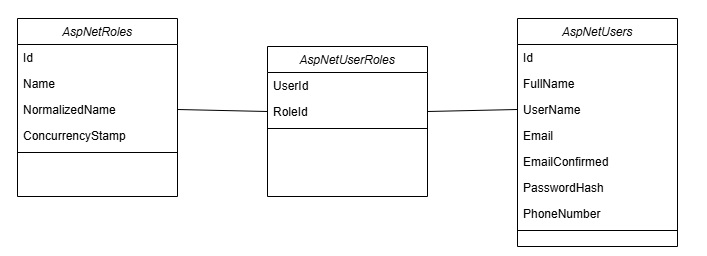
\includegraphics[width=0.8\columnwidth]{DiagClassUsers}
        \caption{Diagramme de classe - Identity User}
        \label{fig:class_users}
    \end{figure}
    
    \item \textbf{Product} : La table \texttt{Product} représente un article destiné à la consommation dans le restaurant.

    \item \textbf{Category} : La table \texttt{Category} permet de classer les produits en différentes catégories afin d'organiser efficacement le menu.

    \item \textbf{Ingredient} : La table \texttt{Ingredient} centralise les informations relatives aux ingrédients utilisés dans les produits. Chaque ingrédient est identifié par un nom. Cette table permet d'associer des ingrédients spécifiques à chaque produit via une relation avec la table \texttt{Product}.

    \item \textbf{Supplement} : La table \texttt{Supplement} contient les informations sur les suppléments associés aux produits. Chaque supplément est défini par un nom et un prix. Cette table facilite la gestion centralisée des suppléments et leur association aux produits via une relation avec la table \texttt{Product}.

    \item \textbf{Image} : La table \texttt{Image} stocke les informations relatives aux images des produits du restaurant. Chaque image peut représenter un plat ou un produit spécifique, afin d'améliorer la présentation visuelle du menu.

    \item \textbf{Drink} : La table \texttt{Drink} répertorie les boissons disponibles dans le restaurant. Elle contient des informations telles que le nom, le prix et d'autres caractéristiques pertinentes. Chaque boisson peut être ajoutée à un panier via la table \texttt{DrinkCart}, permettant ainsi au client de sélectionner une boisson en complément de sa commande.

    \item \textbf{ProductOfTheDay} : La table \texttt{ProductOfTheDay} met en avant un produit spécifique du menu chaque jour, comme une offre spéciale ou un plat du jour. Elle est liée à la table \texttt{Product} via un identifiant (\texttt{ProductId}).

    Le diagramme de classe reliée au gestion du stock peut être représenté de la manière suivante : \\
    \begin{figure}[H]
        \centering
        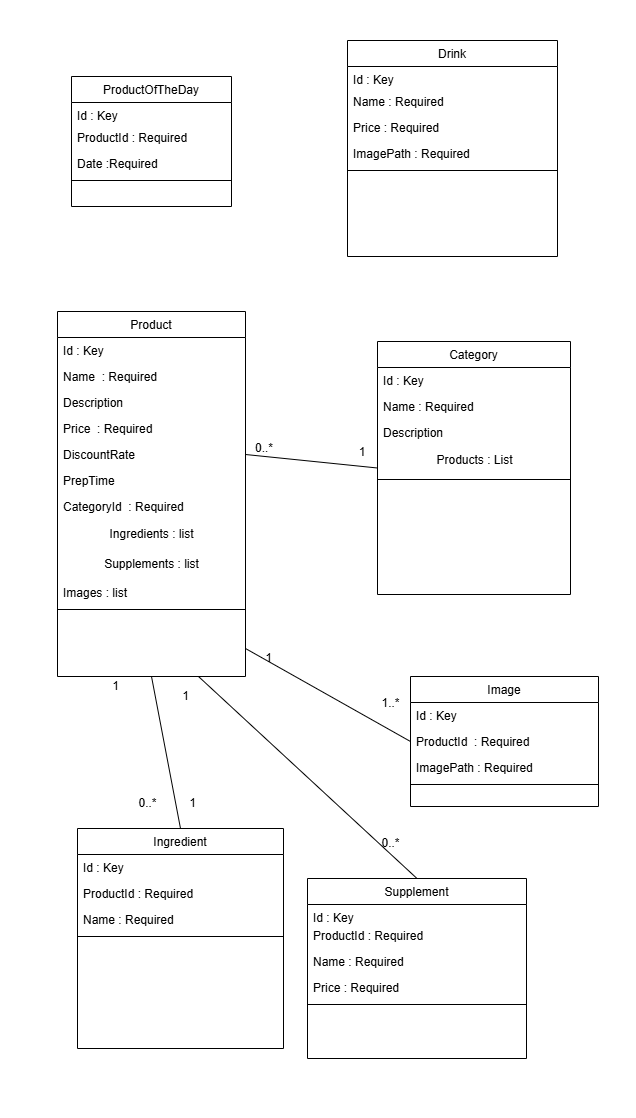
\includegraphics[width=0.8\columnwidth]{DiagClassAdmin}
        \caption{Diagramme de classe - Gestion du stock}
        \label{fig:class_admin}
    \end{figure}
    
    \item \textbf{Cart} : La table \texttt{Cart} représente le panier, qui regroupe l'ensemble des produits et boissons sélectionnés par un client avant la finalisation de la commande.

    \item \textbf{Order} : La table \texttt{Order} représente une commande passée par un client. Elle contient les informations essentielles telles que l'identifiant de la commande, le statut, la date, un message, et l'identifiant du panier associé.


    \item \textbf{ProductCart} : La table \texttt{ProductCart} est utilisée pour gérer les produits ajoutés au panier d'un client. Elle enregistre chaque produit, sa quantité ainsi que ses options supplémentaires (telles que \texttt{ProductCartIngredient} et \texttt{ProductCartSupplement}) lors de la commande. Cette table est liée à la table \texttt{Cart}, ce qui permet de suivre précisément les produits associés à chaque panier.

    \item \textbf{ProductCartIngredient} : La table \texttt{ProductCartIngredient} stocke les ingrédients ajoutés aux produits présents dans le panier.

    \item \textbf{ProductCartSupplement} : La table \texttt{ProductCartSupplement} stocke les suppléments ajoutés aux produits présents dans le panier.

    \item \textbf{DrinkCart} : La table \texttt{DrinkCart} gère la relation entre les boissons et les commandes dans le panier.
    
    Le diagramme de classe reliée au commande et panier peut être représenté de la manière suivante : \\
    \begin{figure}[H]
        \centering
        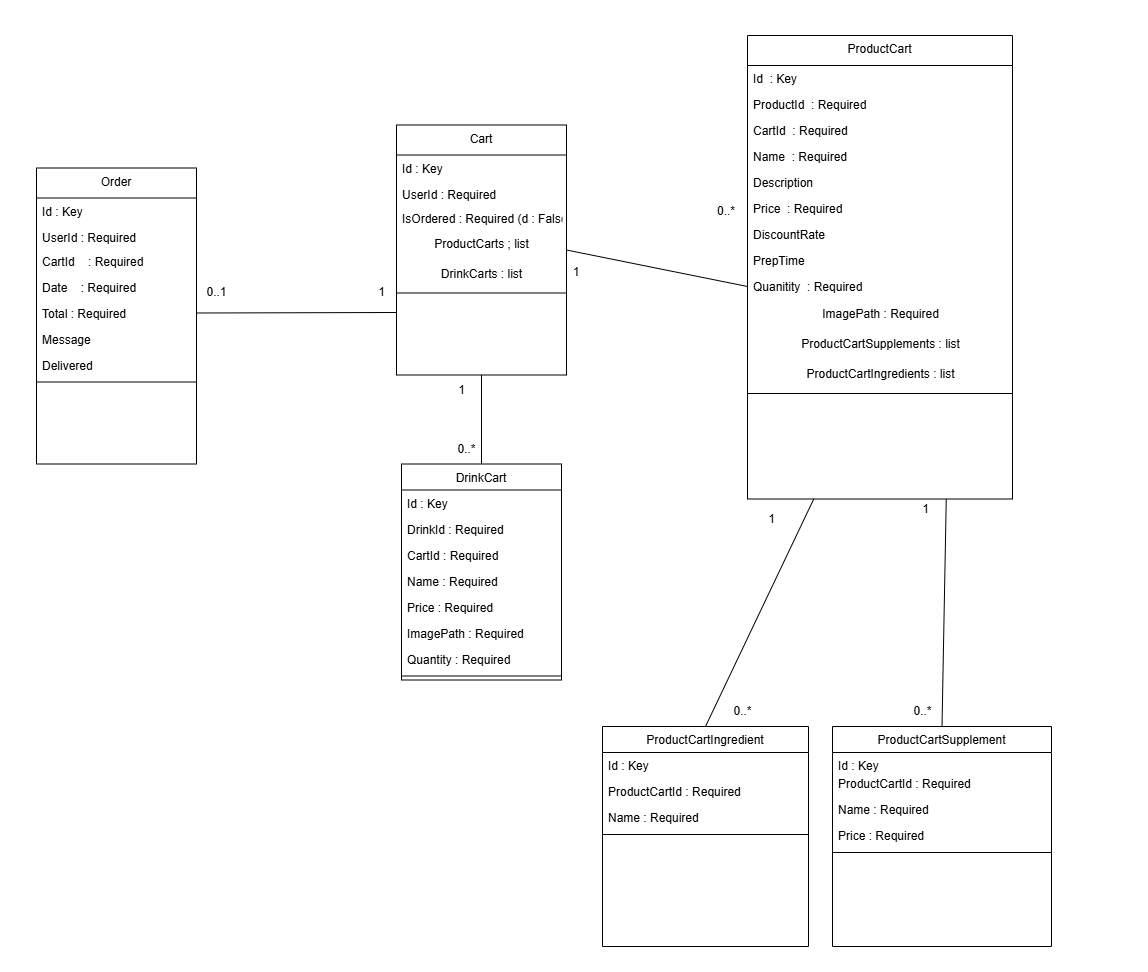
\includegraphics[width=0.8\columnwidth]{DiagClassCart}
        \caption{Diagramme de classe - commande et panier}
        \label{fig:class_cart}
    \end{figure}
    
\end{itemize}
\newpage

\section{Diagramme des cas d’utilisation}
Le diagramme des cas d'utilisation illustre les différentes interactions entre les utilisateurs et l'application, en distinguant les fonctionnalités accessibles à chaque type d'utilisateur. L'application est structurée en deux parties principales : Client et Administrateur.

\section*{Client}
Le diagramme de cas d'utilisation peut être représenté de la manière suivante : \\
\begin{figure}[H]
    \centering
    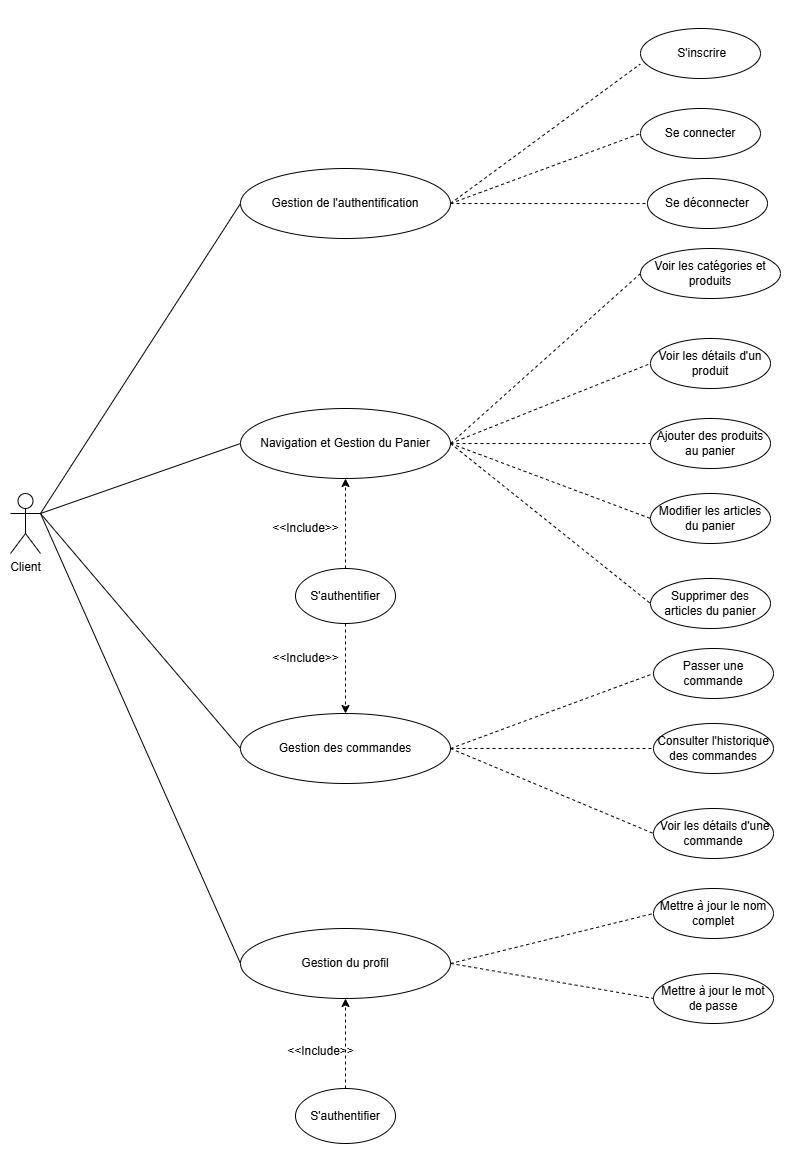
\includegraphics[width=0.7\columnwidth]{DiagUseCaseClient}
    \caption{Diagramme de cas d’utilisation - Client}
    \label{fig:usecase_client}
\end{figure}

\section*{Admin}
Le diagramme de cas d'utilisation peut être représenté de la manière suivante : \\
\begin{figure}[H]
    \centering
    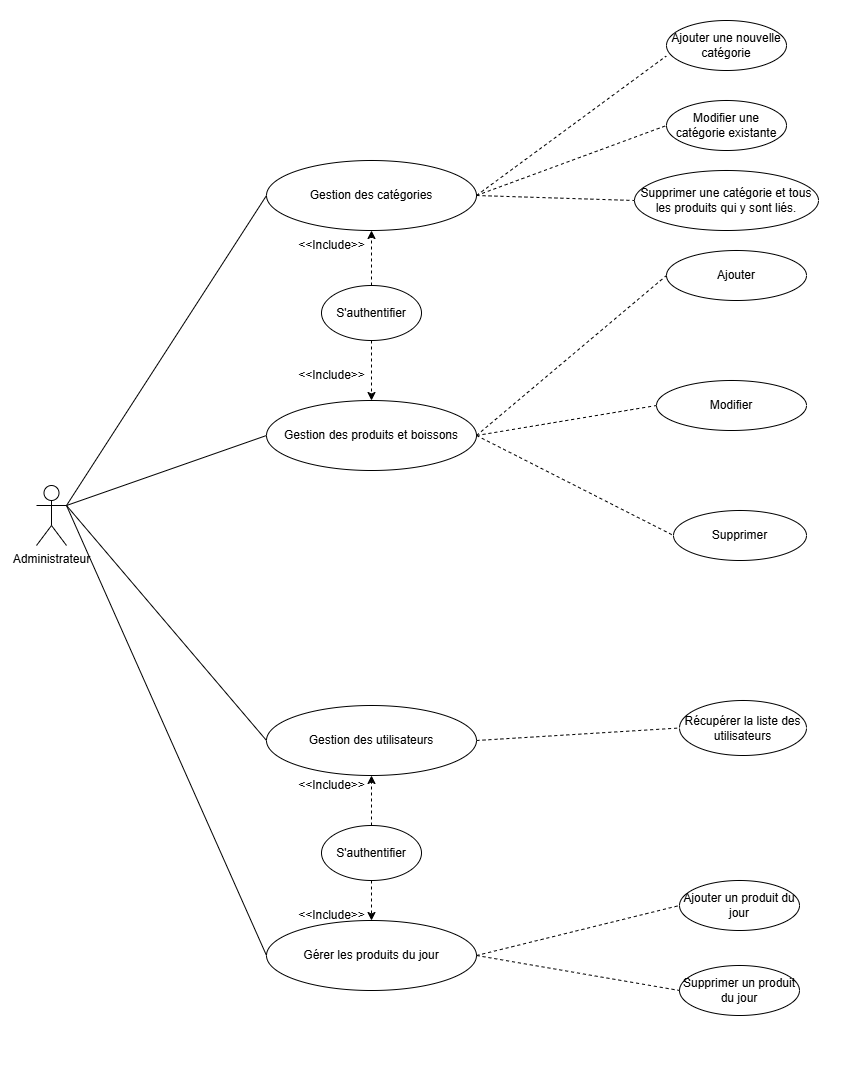
\includegraphics[width=0.8\columnwidth]{DiagUseCaseAdmin}
    \caption{Diagramme de cas d’utilisation - Admin}
    \label{fig:usecase_client}
\end{figure}

\section*{Conclusion}
Les diagrammes de classe et de cas d'utilisation sont essentiels pour modéliser la structure et le comportement de l'application. Ils aident à mieux comprendre les relations entre les entités et les actions possibles pour chaque type d'utilisateur, facilitant ainsi le développement et la maintenance de l'application.



\section{Diagrammes de Séquence}

Les diagrammes de séquence permettent de représenter le déroulement chronologique des interactions entre les utilisateurs (Client et Administrateur) et le système. Ils décrivent l’échange de messages entre les différents composants de l'application pour chaque fonctionnalité clé.

Pour notre application, trois diagrammes principaux sont présentés : l'Authentification, la creation d'un compte client et l'Ajout de produit au panier.

\section*{Authentification}
Le diagramme ci-dessous représente les interactions permettant à un utilisateur (Client ou Administrateur) de s'authentifier dans l'application :

\begin{figure}[H]
    \centering
    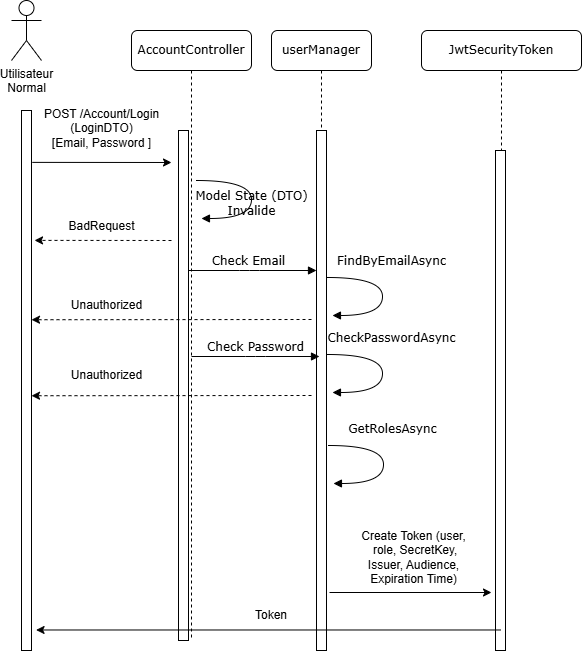
\includegraphics[width=0.5\columnwidth]{DiagSeqAuth}
    \caption{Diagramme de séquence - Authentification}
    \label{fig:seq_auth}
\end{figure}

\section*{Création du compte client}
Le diagramme ci-dessous représente les différentes étapes permettant à un client de créer un compte dans l'application :  
\begin{figure}[H]
    \centering
    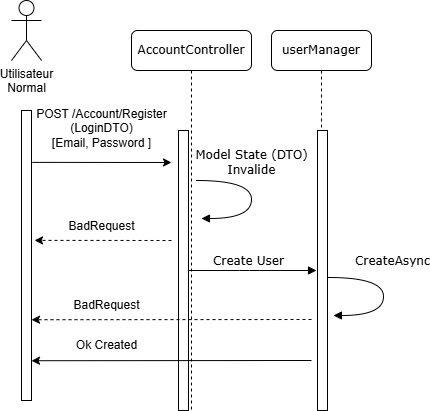
\includegraphics[width=0.5\columnwidth]{DiagSeqRegister}
    \caption{Diagramme de séquence - Création de compte client}
    \label{fig:seq_register}
\end{figure}

\section*{Ajout d'un produit au panier du client}
Le diagramme suivant illustre les interactions liées à l'ajout d'un produit dans le panier du client :  
\begin{figure}[H]
    \centering
    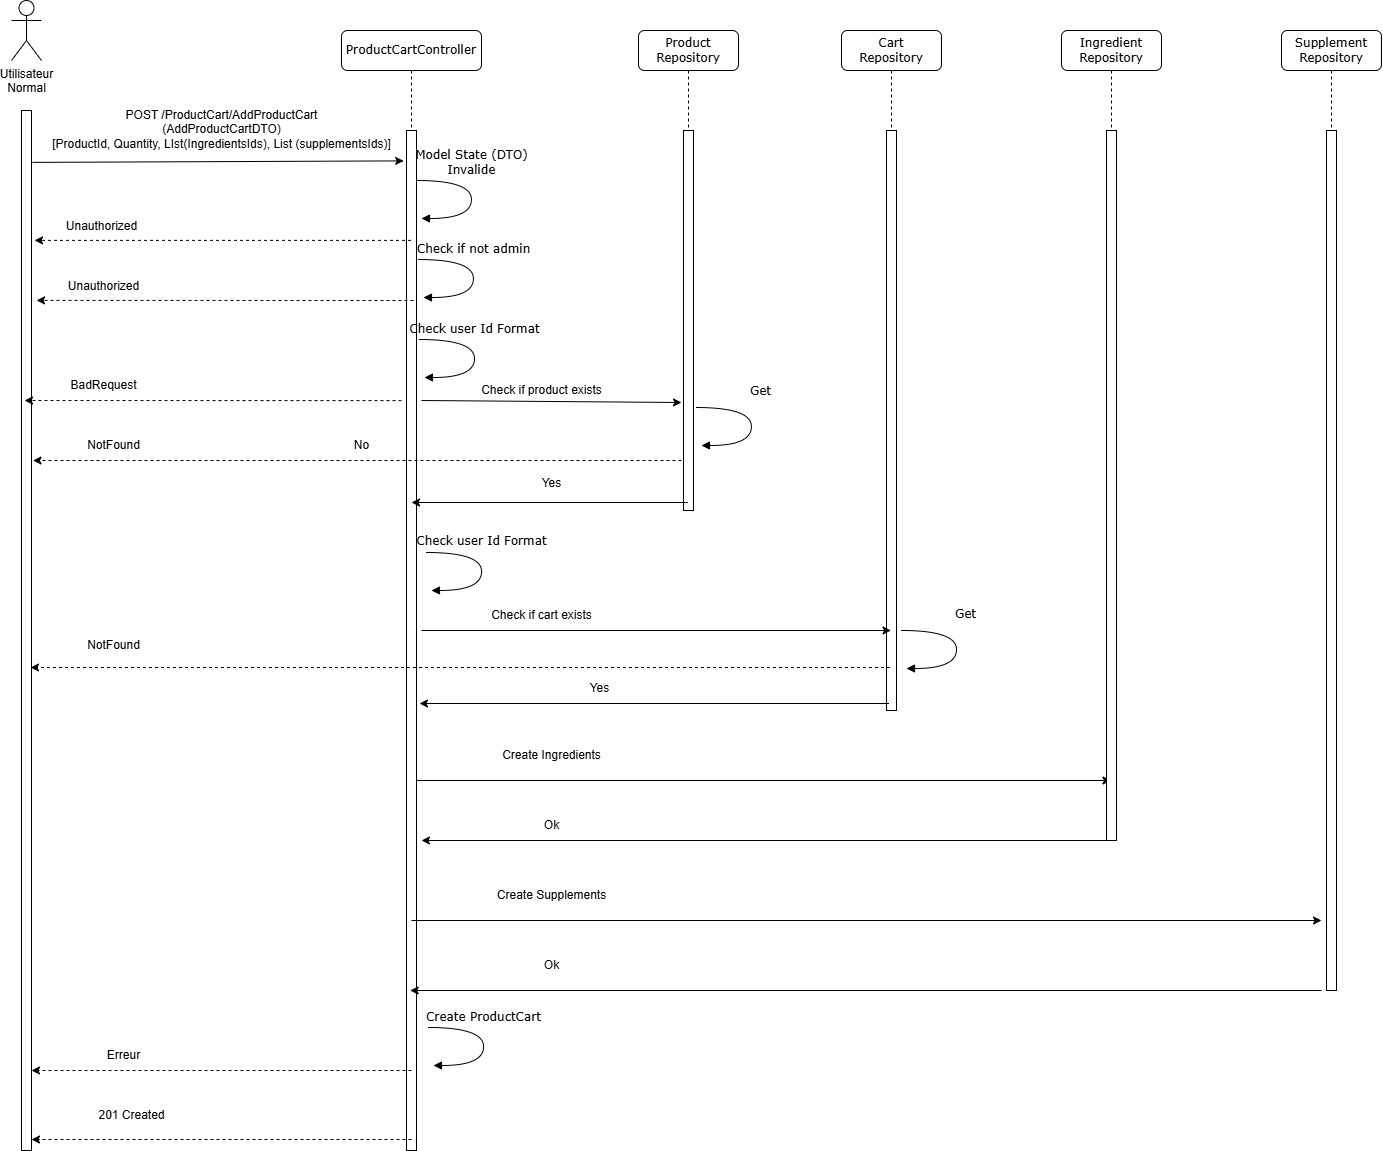
\includegraphics[width=0.8\columnwidth]{DiagSeqAddProductCart}
    \caption{Diagramme de séquence - Ajout d'un produit au panier}
    \label{fig:seq_addtocart}
\end{figure}


\section*{Conclusion}

Les diagrammes de séquence présentés illustrent les interactions clés entre les utilisateurs (Client et Administrateur) et le système. Le diagramme d'authentification montre le processus de connexion des utilisateurs. Celui de la création de compte client décrit l'enregistrement d'un nouvel utilisateur. Enfin, le diagramme d'ajout d'un produit au panier présente l'interaction du client avec le système pour ajouter des produits. Ces diagrammes permettent de visualiser le flux des interactions et la communication entre les différents composants de l'application.

\clearpage

\chapter{Réalisation et Resultats}


\section{Architecture de l'Application}

L'application suit une architecture client-serveur pour garantir modularité et évolutivité.
\begin{itemize}
    \item \textbf{Frontend} :  
    Le frontend est développé en \textbf{ReactJS}, un framework JavaScript qui permet de concevoir des interfaces interactives et réactives. Il communique avec le backend via des appels API.

    \item \textbf{Backend} :  
    Le backend est implémenté en \textbf{ASP.NET API}, qui gère la logique métier, les interactions avec la base de données, et les points d’accès pour le frontend.  
    Pour structurer le backend, les patterns Repository et IRepository ont été adoptés afin d'assurer une séparation claire des responsabilités et de simplifier la maintenance.

    \item \textbf{Base de données} :  
    SQL Server est utilisé pour assurer un stockage structuré et fiable des données.

    \item \textbf{IDE} :  
    Visual Studio et Visual Studio Code offrent un environnement de développement intuitif pour le backend et le frontend.
\end{itemize}

\section{Présentation des principaux endpoints}

Dans le cadre de l’application de gestion des commandes de restaurant, plusieurs endpoints API ont été développés pour gérer les différentes fonctionnalités de l’application. Ces endpoints permettent d’interagir avec les données du système telles que l’authentification des utilisateurs, la gestion des commandes, et la consultation du menu. Voici une liste des principaux endpoints API développés :

\subsection*{Compte (Account)}
\begin{itemize}
    \item \textbf{POST} /api/Account/Register : Inscription d'un nouvel utilisateur. Permet de créer un compte en envoyant les informations nécessaires (nom complet, email, mot de passe).
    \item \textbf{POST} /api/Account/Login : Authentification. Retourne un JWT à utiliser pour sécuriser les requêtes futures.
    \item \textbf{POST} /api/Account/ChangePassword : Permet de modifier le mot de passe de l'utilisateur authentifié.
    \item \textbf{POST} /api/Account/ChangeFullName : Permet de mettre à jour le nom complet de l'utilisateur.
    \item \textbf{GET} /api/Account/GetUsers : Retourne la liste de tous les utilisateurs (accessible avec des permissions spécifiques, par exemple pour un administrateur).
    \item \textbf{GET} /api/Account/GetUser : Retourne les détails de l'utilisateur authentifié.
\end{itemize}

\subsection*{Panier (Cart)}
\begin{itemize}
    \item \textbf{POST} /api/Cart/AddCart : Crée un nouveau panier pour l'utilisateur authentifié.
    \item \textbf{GET} /api/Cart/GetCart : Récupère les détails du panier de l'utilisateur.
    \item \textbf{PUT} /api/Cart/EditCart : Modifie les informations du panier (ajout ou suppression de produits, par exemple).
\end{itemize}

\subsection*{Catégories (Category)}
\begin{itemize}
    \item \textbf{POST} /api/Category/AddCategory : Ajoute une nouvelle catégorie de produits (accessible aux administrateurs).
    \item \textbf{GET} /api/Category/GetCategory/{Id} : Récupère les détails d'une catégorie spécifique.
    \item \textbf{GET} /api/Category/GetAllCategories : Récupère toutes les catégories disponibles.
    \item \textbf{PUT} /api/Category/EditCategory/{Id} : Modifie une catégorie existante.
    \item \textbf{DELETE} /api/Category/DeleteCategory/{Id} : Supprime une catégorie existante.
\end{itemize}

\subsection*{Produits (Product)}
\begin{itemize}
    \item \textbf{POST} /api/Product/AddProduct : Ajoute un nouveau produit (accessibles aux administrateurs).
    \item \textbf{GET} /api/Product/GetProduct/{Id} : Récupère les détails d'un produit spécifique.
    \item \textbf{GET} /api/Product/GetAllProducts : Récupère tous les produits disponibles.
    \item \textbf{GET} /api/Product/GetProductsByCategory/{CategoryId} : Récupère les produits liés à une catégorie spécifique.
    \item \textbf{PUT} /api/Product/EditProduct/{Id} : Modifie les détails d'un produit existant.
    \item \textbf{DELETE} /api/Product/DeleteProduct/{Id} : Supprime un produit existant.
\end{itemize}

\subsection*{Commandes (Order)}
\begin{itemize}
    \item \textbf{POST} /api/Order/AddOrder : Crée une nouvelle commande en envoyant les détails (produits, quantités, etc.).
    \item \textbf{GET} /api/Order/GetOrder/{Id} : Récupère les détails d'une commande spécifique.
    \item \textbf{GET} /api/Order/GetUserOrders : Récupère toutes les commandes passées par l'utilisateur authentifié.
    \item \textbf{GET} /api/Order/GetAllOrders : Récupère toutes les commandes (accessible aux administrateurs).
    \item \textbf{PUT} /api/Order/EditOrder/{Id} : Met à jour les détails d'une commande spécifique.
    \item \textbf{DELETE} /api/Order/DeleteOrder/{Id} : Supprime une commande existante.
    \item \textbf{PUT} /api/Order/Deliver/{Id} : Met à jour le statut d'une commande pour la marquer comme livrée.
\end{itemize}

\subsection*{Boissons (Drink) et Produits du jour (ProductOfTheDay)}
Ces endpoints suivent des schémas similaires, avec des options pour ajouter, récupérer, modifier ou supprimer des éléments.

\section{Fonctionnement des principaux endpoints}

\subsection*{POST /api/Account/Login}
L'utilisateur envoie ses informations d'identification (email et mot de passe) dans une requête POST. En cas de succès, un JWT est généré et retourné dans la réponse. Ce jeton doit être inclus dans l'en-tête \textbf{Authorization} des requêtes nécessitant une authentification.

\subsection*{GET /api/Order/GetUserOrders}
Ce point d'accès permet aux utilisateurs authentifiés de récupérer la liste de leurs commandes. Si le JWT est valide, la liste est renvoyée ; sinon, une réponse HTTP 401 Unauthorized est retournée.

\subsection*{POST /api/Order/AddOrder}
Les utilisateurs peuvent créer une commande en envoyant les détails (produits, quantités) dans une requête POST. Le JWT est utilisé pour authentifier et associer la commande à l'utilisateur.

\subsection*{PUT /api/Order/EditOrder/{Id}}
Les utilisateurs peuvent modifier leurs commandes en fournissant l'ID de la commande à mettre à jour et les nouvelles informations. Le JWT est vérifié pour garantir que seul l'utilisateur propriétaire ou un administrateur puisse effectuer cette modification.

\subsection*{GET /api/Product/GetAllProducts}
Ce point d'accès est ouvert pour récupérer la liste de tous les produits disponibles. Certaines fonctionnalités supplémentaires, comme le filtrage par catégorie, peuvent être implémentées.

\section{Sécurisation des endpoints}

\subsection*{Authentification avec JWT}
Le système d'authentification utilise des tokens JWT générés lors de la connexion. Ces jetons permettent de valider l'identité de l'utilisateur pour toutes les requêtes subséquentes.

\subsection*{Middleware de validation}
Un middleware assure la validation des JWT. Si le token est absent ou invalide, l'accès à l'endpoint est refusé.

\subsection*{Contrôle d'accès basé sur les rôles}
Certains endpoints, comme ceux liés à la gestion des produits ou des catégories, sont restreints aux administrateurs grâce à des rôles inclus dans le JWT.

\subsection{Création du compte Admin}
Lors du lancement de l'application, un compte \textit{Admin} est créé automatiquement, avec l'assignation d'un rôle d'utilisateur \textit{Admin}. Cela permet à l'administrateur d'accéder aux fonctionnalités de gestion, telles que l'ajout, la modification ou la suppression de produits, la gestion des catégories et des utilisateurs, etc.

\section{Évolutions possibles}

Plusieurs améliorations et nouvelles fonctionnalités sont prévues pour enrichir l’application et offrir une expérience utilisateur encore plus fluide et complète :

\begin{itemize}
    \item \textbf{Suivi des commandes en temps réel :} Une fonctionnalité permettant aux utilisateurs de suivre en temps réel l'état de leur commande, depuis la préparation jusqu'à la livraison. Cela ajoutera une couche de transparence et de confort pour l'utilisateur.
    
    \item \textbf{Gestion des paiements en ligne :} L'intégration d'une solution de paiement en ligne permettra aux utilisateurs de régler leurs commandes directement via l'application, simplifiant ainsi le processus d'achat et améliorant l'expérience utilisateur.
    
    \item \textbf{Intégration avec des services de livraison :} Cette fonctionnalité permettra une gestion complète des commandes, y compris l'expédition et la livraison des produits. L'intégration avec des services tiers de livraison offrira une solution tout-en-un, améliorant ainsi l'efficacité et la satisfaction client.
\end{itemize}
Ces évolutions viseront à rendre l'application plus pratique, complète et compétitive sur le marché, tout en répondant mieux aux besoins des utilisateurs.

\clearpage


\section*{Conclusion}

En conclusion, l'application de gestion des commandes de restaurant que nous avons développée représente une solution complète et moderne pour la gestion des commandes, de l'authentification des utilisateurs et a la consultation du menu. Cette application a été conçue pour répondre à un besoin spécifique dans le domaine de la restauration, en facilitant la prise de commande en ligne et la gestion des données utilisateurs dans un environnement sécurisé.

L'implémentation de l'authentification basée sur JWT (JSON Web Token) assure une gestion fluide et sécurisée des sessions utilisateurs, tout en garantissant que seules les requêtes authentifiées peuvent accéder aux ressources protégées de l'application. Le processus d'authentification est non seulement sécurisé, mais aussi évolutif, permettant à l'application de supporter une base d'utilisateurs croissante sans nécessiter de stockage des sessions côté serveur.

Le Repository Pattern a été appliqué pour maintenir une séparation claire entre la logique métier et la gestion des données. Cela permet une meilleure organisation du code, une facilité de maintenance et une meilleure testabilité des différentes parties de l'application. L'utilisation de ce pattern a permis de centraliser l'accès aux données et de simplifier les opérations CRUD pour les entités principales.

Les différents endpoints de l'API ont été soigneusement développés pour répondre aux besoins des utilisateurs, tout en offrant une interface claire et intuitive pour l'administration et les clients. La sécurisation des endpoints par JWT et la gestion des rôles d'utilisateur (comme l'administrateur et les client) assurent une utilisation sécurisée et flexible de l'application.

De plus, les diagrammes de classe et de cas d'utilisation ont permis de clarifier la structure de l'application, illustrant les relations entre les entités et les principales interactions entre les acteurs du système. Ces diagrammes ont facilité la compréhension du fonctionnement interne de l'application et ont guidé le développement des différentes fonctionnalités.

En somme, cette application démontre l'importance d'une architecture solide et d'une gestion sécurisée des données dans les applications modernes, en particulier celles qui manipulent des informations sensibles. Avec une bonne base en place, il est possible d'ajouter de nouvelles fonctionnalités, comme des systèmes de notifications ou des modules de recommandation pour améliorer l'expérience client. L'utilisation de technologies robustes et la mise en œuvre des meilleures pratiques garantissent la pérennité et la scalabilité de l'application à long terme.

\clearpage

\end{document}